\clearpage
\section{Benutzeroberflächen}

\subsection{DISPO}

DISPO bleibt die primäre Arbeitsoberfläche des Disponenten. Dort befinden sich Auftragsliste,
Tourplanung, Karte und Lieferdetails (siehe Abbildung~\ref{fig:dispo-overview}). Für die
Integration werden ein Auslöser pro Auftrag und eine kompakte Rückmeldestatusanzeige
vorgeschlagen. Position und Symbolik sind noch mit dem DISPO-Produktteam festzulegen.

\subsection{Bestätigungsseite}

Die Kundenansicht konzentriert sich auf Lieferdatum, Zeitfenster und die wichtigsten
Auftragsdaten. Bestätigen und Ablehnen sind als eindeutige Aktionen vorgesehen. Die folgende
Abbildung zeigt den aktuellen Mock mit fiktiven Beispieldaten; der untere Teil der Seite ist
für diese Übersicht ausgeblendet.

\subsection{Avisierungsdashboard}

Die Hauptansicht stellt Aufträge nach Tour gruppiert dar und macht ihren Rückmeldestatus
unmittelbar unterscheidbar. Suche sowie Filter nach Status und Tour unterstützen den
Disponenten dabei, offene oder problematische Fälle gezielt zu finden.

Die Detailansicht zeigt den konkreten Auftrag, die Kundenantwort und die weitere Bearbeitung.
Der aktuelle Mock veranschaulicht au\ss{}erdem die Wahl eines Kommunikationskanals. Die endgültige
Bedienlogik wird mit dem fachlichen Prozess und der DISPO-Integration abgestimmt.

\clearpage
\begin{landscape}
\thispagestyle{plain}
\begin{figure}[p]
  \centering
  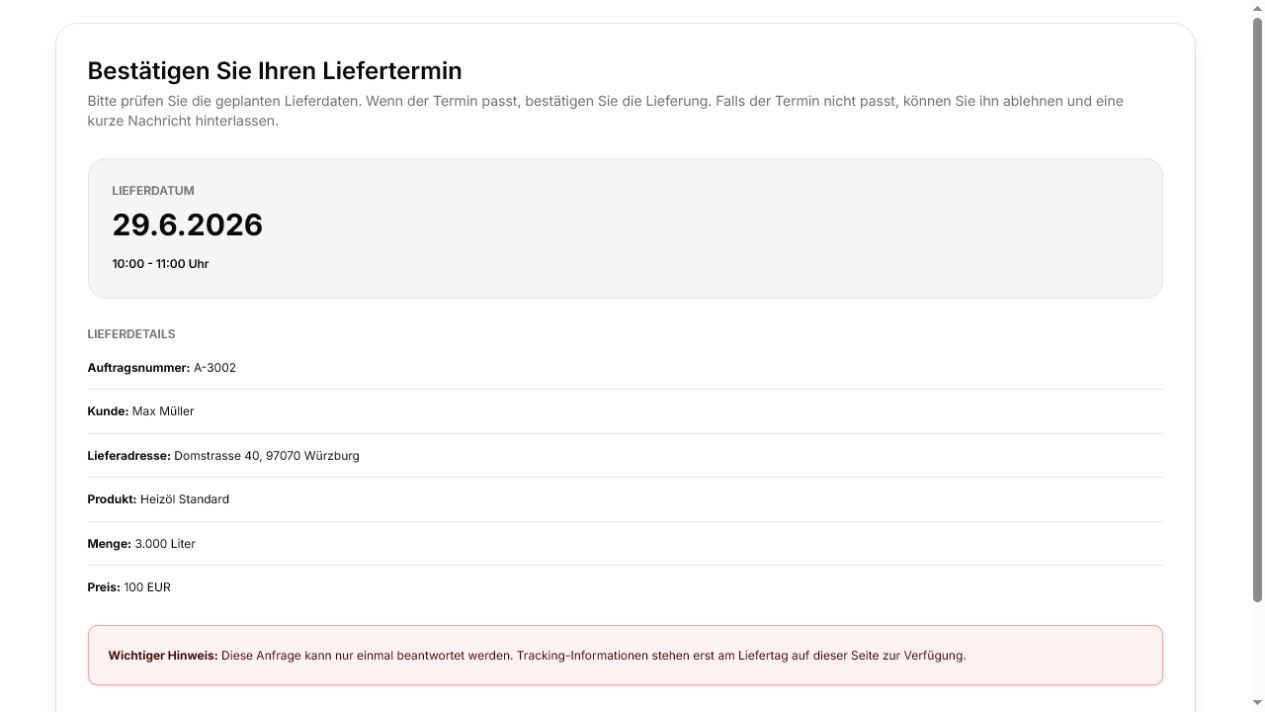
\includegraphics[width=\linewidth,height=0.88\textheight,keepaspectratio,trim=0 100 0 0,clip]{assets/screenshots/bestaetigungsseite.png}
  \caption{Bestätigungsseite des Kunden im aktuellen Mock}
  \label{fig:confirmation-ui}
\end{figure}
\end{landscape}
\clearpage

\begin{landscape}
\thispagestyle{plain}
\begin{figure}[p]
  \centering
  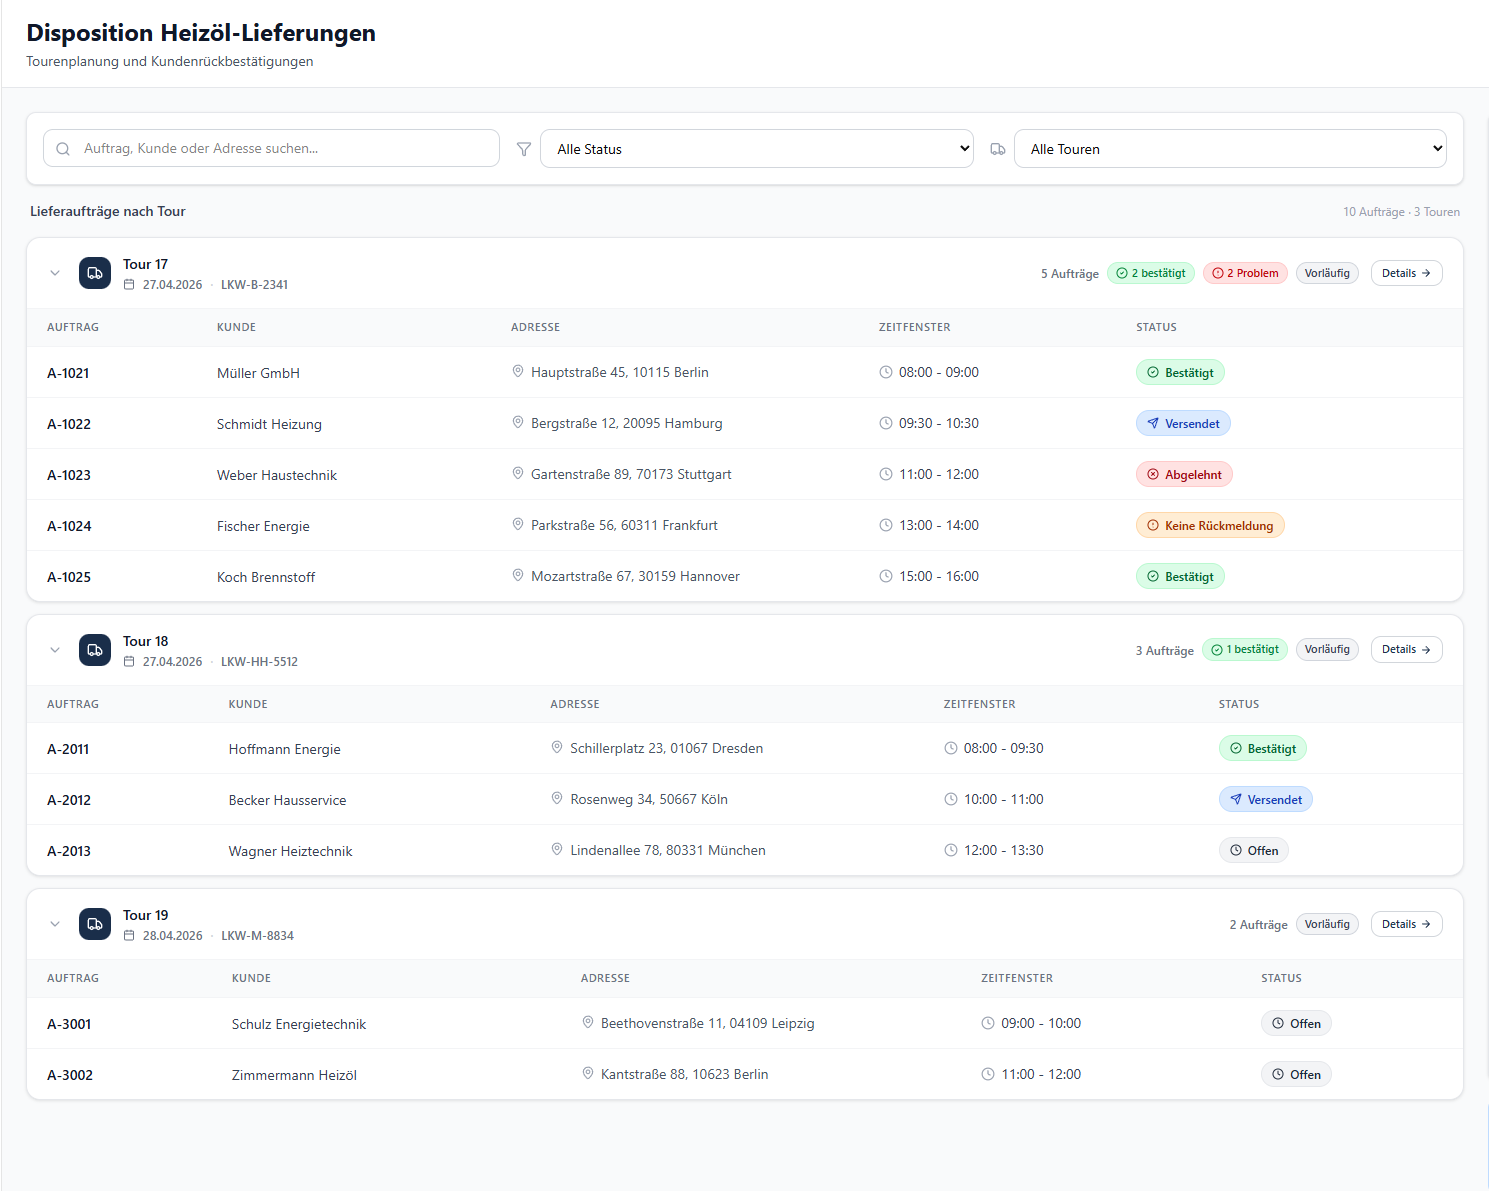
\includegraphics[width=\linewidth,height=0.88\textheight,keepaspectratio,trim=0 210 0 0,clip]{assets/screenshots/avisierungsdashboard-touren.png}
  \caption{Avisierungsdashboard mit Filterung und nach Tour gruppierten Aufträgen}
  \label{fig:dashboard-ui}
\end{figure}
\end{landscape}
\clearpage

\begin{landscape}
\thispagestyle{plain}
\begin{figure}[p]
  \centering
  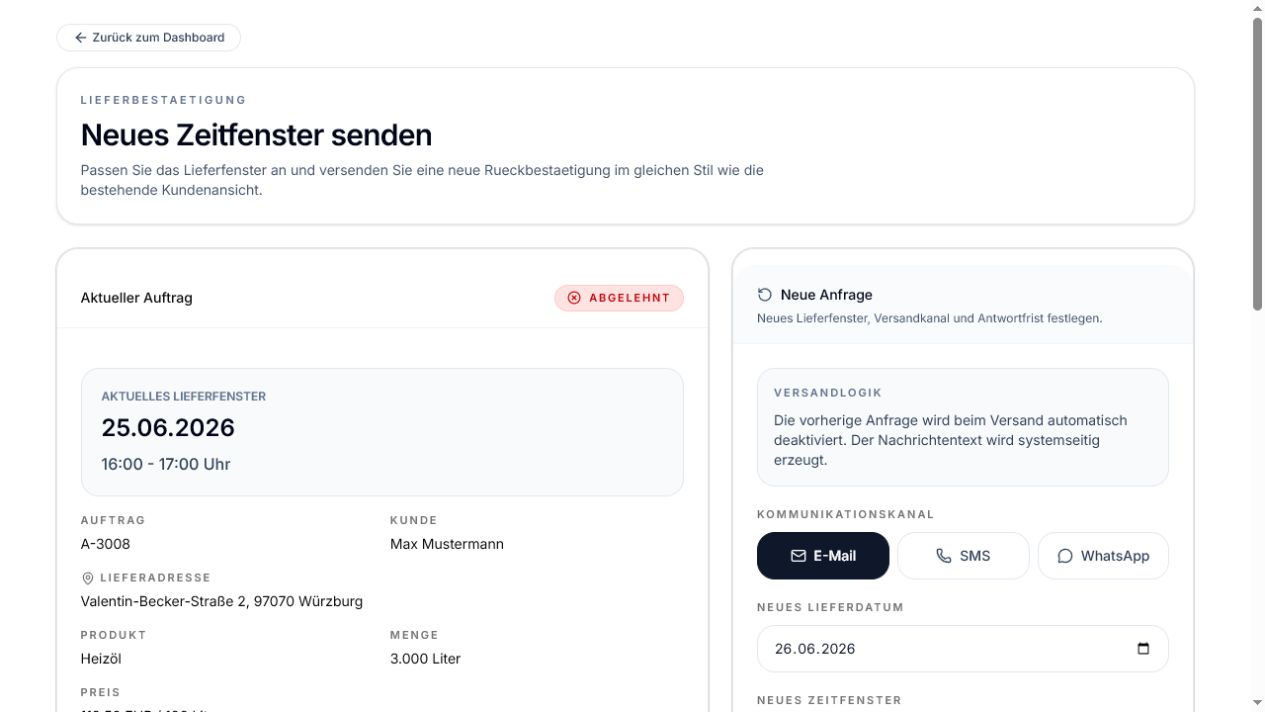
\includegraphics[width=\linewidth,height=0.88\textheight,keepaspectratio]{assets/screenshots/avisierungsdashboard-detail.png}
  \caption{Detailansicht eines abgelehnten Falls im aktuellen Mock}
  \label{fig:dashboard-detail-ui}
\end{figure}
\end{landscape}
\clearpage
